\chapter{Arquitetura do Sistema}\label{cap:arquitetura}

Este capítulo descreve como a ferramenta desenvolvida interage com os
\textit{softwares} em uso na competição.

Os seguintes \textit{softwares} externos são de relevância para o entendimento
da arquitetura escolhida:

\begin{itemize}
  \item ssl-vision: desenvolvido pela comunidade e de uso oficial na competição
    para processamento das imagens da câmera nas partidas e distribuição pela
    rede dos dados processados (estado do jogo);
  \item grSim: desenvolvido pela comunidade e amplamente usado pelas equipes
    para simular o ambiente das partidas, o protocolo usado para enviar o estado
    pela rede é identico ao do ssl-vision;
  \item pyroboime: também chamado de core desenvolvido pela RoboIME, atualmente
    provê uma camada de abstração sobre a comunicação com o ambiente de jogo
    (real ou simulado) incluindo redução de ruído, planejamento de trajetória e
    controle.
\end{itemize}

Para fins práticos o desenvolvimento ocorre com validações no simulador (grSim).
O comportamento é compatível com as partidas oficiais.

\section{Comunicação com Componentes Externos}

\begin{figure}[H]
  \centering
  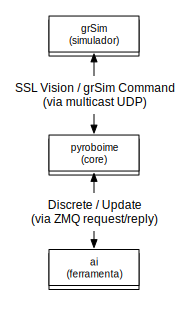
\includegraphics[height=10cm]{communication}
  \caption{Diagrama de comunicação entre os componentes.}\label{fig:arch-comm}
\end{figure}

A figura~\ref{fig:arch-comm} representa como os componentes se comunicam.  A
ferramenta se comunica apenas com o pyroboime para aproveitar todas as
funcionalidades necessárias que fogem ao escopo desse trabalho.  Por isso o foco
do desenvolvimento está concentrado em atender diretamente os objetivos.

As mensagens trocadas entre a ferramenta e o core (\textit{pyroboime}) é
codificada com o \textit{Protobuf}, uma biblioteca bem estabelecida que também é
usada nos protocolos oficiais da competição.  Desse modo o \textit{overhead} de
comunicação é baixo, não é necessário introduzir uma dependência ou codificação
manual no core e é possível que versões futuras sejam retrocompatíveis.

São dois tipos de mensagens:

\begin{itemize}
  \item atualização do estado: sentido do core para a ferramenta, codificadas
    com a mensagem UpdateMessage, descreve todas as informações necessárias para
    criar um estado novo;
  \item comando de ações: sentido ferramenta para o core, codificadas com a
    mensagem CommandMessage, descreve a ação que cada agente (robô) deve
    realizar.
\end{itemize}

As especificações de ambas as mensagens se encontram no anexo~\ref{att:protos}.

As mensagens são transmitidas num socket ZMQ (\textit{ZeroMQ}, uma biblioteca de
transmissão de dados na rede) visando a extensibilidade da ferramenta, pois com
tal biblioteca é possível distribuir mensagens entre vários nós de forma
confiável (característica desejável para um sistema distribuido) além de provêr
confiabilidade e auto-reconexão para o uso atual.

O modo de transmissão é \textit{request-reply} em que a ferramente age como
servidor respondendo as requisições do core, que consistem em atualizações cuja
a resposta deve ser o comando a ser executado naquele estado requisitado.  Na
prática a ferramenta irá transmitir o comando mais recente, que se encontra em
seu \textit{buffer}, descrito brevemente no seção~\ref{sec:threads}.

\section{\textit{Threads} do Sistema}\label{sec:threads}

\begin{figure}[H]
  \centering
  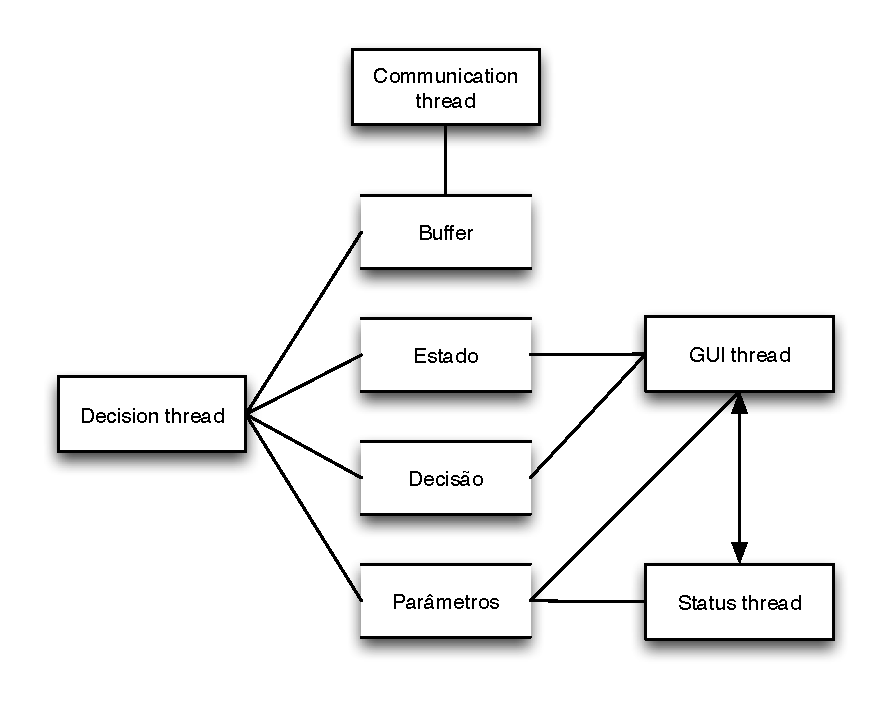
\includegraphics[height=10cm]{threads}
  \caption{Diagrama de relação entre \textit{threads} e
  dados.}\label{fig:arch-threads}
\end{figure}

A ferramenta está implementada em 4 \textit{threads} fixas de acordo com a
figura~\ref{fig:arch-threads}.  A separação foi motivada por:

\begin{itemize}
  \item A interface gráfica necessitar ser responsiva ao usuário;
  \item A taxa de tomada de decisão poder ser mais lenta que a taxa de
    atualização do estado, portanto a comunicação tem sua própria
    \textit{thread} que escreve e lê de um buffer compartilhado pela
    \textit{thread} de tomada de decisão;
  \item Certas informações devem ser coletadas periódicamente para atualizar
    alguns parâmetros e exibidas para o usuário.
\end{itemize}

\section{API Pública}

% TODO: um diagrama de colaboração de classes seria útil aqui

Uma API consiste nas estruturas e funções (ou também métodos) que estão
disponíveis para o programador.  A ferramenta está programada de forma que
também é possível fazer o uso programático de suas funcionalidades.

Esta seção descreve com detalhes cada estrutura e função presente na API da
ferramenta.  É um objetivo desta seção documentar o código da ferramenta para
possibilitar a evolução dessa em projetos futuros ou integração em outros
projetos.

Todas as estruturas e funções estão expostas em \textit{headers} C++, porém esta
documentação irá tratar apenas das funcionalidades e organização sem prender à
sintaxe ou modo de uso na linguagem em que está programada.  Para tais detalhes
o anexo~\ref{att:headers} pode ser consultado, esse contém o conteúdo dos
headers tratados nesta seção.

\subsection*{Enumeração \textit{ActionType}}

Representa o tipo da ação.

\subsubsection*{Alternativas}

\begin{itemize}
  \item \textit{NONE}: nenhuma ação;
  \item \textit{MOVE}: acão de movimentação;
  \item \textit{PASS}: ação de passe;
  \item \textit{KICK}: ação de chute.
\end{itemize}

\subsection*{Estrutura \textit{Action}}

Representa a ação individual a ser executada por um robô, não está amarrada à um
robô, essa associação deve ser feita pelo usuário da estrutura, isso permite uma
associação implicita baseada na ordem do vetor ou outros tipos de otimizações,
por esse motivo algumas funções recebem um Id de robô para saber qual robô usar
em certas circunstâncias.

\subsubsection*{Atributos}

\begin{itemize}
  \item \textit{type}: tipo (\textit{ActionType}), por padrão é do tipo NONE;
  \item \textit{move_pos}: posição destino da movimentação;
  \item \textit{kick_pos}: posição alvo do chute;
  \item \textit{pass_receiver}: Id do robô que deve receber o passe.
\end{itemize}

\subsubsection*{Métodos}

\begin{itemize}
  \item \textit{make_move_action}
    \par Entrada: vetor indicando um destino.
    \par Saída: ação do tipo MOVE.
  \item \textit{make_kick_action}
    \par Entrada: vetor indicando um alvo.
    \par Saída: ação do tipo KICK.
  \item \textit{make_pass_action}
    \par Entrada: Id de robô, que irá receber o passe.
    \par Saída: ação do tipo PASS.
  \item \textit{gen_move_action}
    \par Entrada: Id de um robô, estado, tabela de decisão.
    \par Saída: ação do tipo MOVE aleatória, que não colide com a posição de
    nenhum outro robô, nem com a posição destino desses de acordo com a tabela
    de decisão.
  \item \textit{gen_kick_action}
    \par Entrada: Id de um robô, estado, tabela de decisão.
    \par Saída: ação do tipo KICK no ponto de maior abertura do gol do inimigo
    que continuar aberto após as movimentações da tabela de decisão.  É assumido
    que um chute é possível e isso foi verificado previamente.
  \item \textit{gen_pass_action}
    \par Entrada: Id de um robô, estado, tabela de decisão.
    \par Saída: ação do tipo PASS aleatória para algum robô (do mesmo time) que
    possa receber o passe, o critério para receber o passe envolve que o
    receptor chegue em seu destino antes que o passador consiga chegar na bola e
    chuta-lá até o destino do receptor, além disso após o chute o receptor deve
    conseguir ser o dono da bola.
  \item \textit{gen_primary_action}
    \par Entrada: Id de um robô, estado, tabela de decisão, flag que indica se é
    de chute.
    \par Saída: ação do tipo KICK ou PASS, simplesmente abstrai
    \textit{gen_pass_action} ou \textit{gen_kick_action} para evitar verbosidade.
  \item \textit{apply_to_state}
    \par Entrada: ação, Id do robô, referência para um estado.
    \par Efeito: aplica a ação a um estado.  É assumido que a ação pode ser
    aplicada.  Ações de chute levam a bola para o gol.
\end{itemize}

%#ifndef CONSTS_H
%#define CONSTS_H
%
%constexpr int N_ROBOTS = 6;
%constexpr int MAX_SUGGESTIONS = 30;
%constexpr int MAX_SUGGESTION_SPOTS = 30;
%
%// Units are SI: m, m/s, s, ...
%
%constexpr float LINE_WIDTH = 0.010;
%constexpr float FIELD_WIDTH = 8.090;
%constexpr float FIELD_HEIGHT = 6.050;
%constexpr float GOAL_WIDTH = 1.000;
%constexpr float GOAL_DEPTH = 0.180;
%constexpr float GOAL_WALL_WIDTH = 0.020;
%constexpr float CENTER_CIRCLE_RADIUS = 0.500;
%constexpr float DEFENSE_RADIUS = 1.000;
%constexpr float DEFENSE_STRETCH = 0.500;
%constexpr float BOUNDARY_WIDTH = 0.500;
%constexpr float REFEREE_WIDTH = 0.250;
%constexpr float ROBOT_RADIUS = 0.180 / 2;
%constexpr float BALL_RADIUS = 0.043 / 2;
%constexpr float ROBOT_MAX_SPEED = 1.0;
%constexpr float ROBOT_KICK_SPEED = 6.0;
%constexpr float MAX_PASS_DISTANCE = 2.5;
%
%constexpr const char *PROGRAM_NAME =
%    "AI for RoboIME"; // TODO: better name maybe?
%constexpr int GUI_DEFAULT_WIDTH = 944;
%constexpr int GUI_DEFAULT_HEIGHT = 740;
%
%enum _ParamGroup {
%  MAX_ATTACK = 0,
%  MIN_ATTACK = 1,
%  MAX_CONQUER = 2,
%  MIN_CONQUER = 3
%};
%
%extern const int *const PARAM_GROUP;
%extern bool PARAM_GROUP_AUTOSELECT;
%extern bool PARAM_GROUP_CONQUER;
%extern float PARAM_GROUP_THRESHOLD;
%extern float PARAM_GROUP_CONQUER_TIME;
%void set_param_group(int new_param_group);
%
%#ifdef _CONST_IMPL
%#define PARAM(TYPE, NAME, DEFAULT) _CONST_IMPL(TYPE, NAME, DEFAULT)
%#else
%#define PARAM(TYPE, NAME, DEFAULT) extern TYPE NAME;
%#endif
%
%PARAM(bool, CONSTANT_RATE, true);
%PARAM(bool, KICK_IF_NO_PASS, false);
%PARAM(int, DECISION_RATE, 7);
%PARAM(int, RAMIFICATION_NUMBER, 5000);
%PARAM(int, FULL_CHANGE_PERCENTAGE, 100);
%PARAM(int, MAX_DEPTH, 0);
%PARAM(float, KICK_POS_VARIATION, 0.150);
%PARAM(float, MIN_GAP_TO_KICK, 18.0);
%PARAM(float, DESIRED_PASS_DIST, 2.0);
%PARAM(float, WEIGHT_BALL_POS, 0);
%PARAM(float, WEIGHT_MOVE_DIST_MAX, 0);
%PARAM(float, WEIGHT_MOVE_DIST_TOTAL, 0);
%PARAM(float, WEIGHT_MOVE_CHANGE, 2);
%PARAM(float, WEIGHT_PASS_CHANGE, 2);
%PARAM(float, WEIGHT_KICK_CHANGE, 2);
%PARAM(float, TOTAL_MAX_GAP_RATIO, 0.5);
%PARAM(float, WEIGHT_CLOSE_TO_BALL, 1000);
%PARAM(float, WEIGHT_ENEMY_CLOSE_TO_BALL, 1000);
%PARAM(float, WEIGHT_HAS_BALL, 5000);
%PARAM(float, WEIGHT_ATTACK, 1000);
%PARAM(float, WEIGHT_SEE_ENEMY_GOAL, 10);
%PARAM(float, WEIGHT_BLOCK_GOAL, 180);
%PARAM(float, WEIGHT_BLOCK_ATTACKER, 5000);
%PARAM(float, WEIGHT_GOOD_RECEIVERS, 0);
%PARAM(float, WEIGHT_RECEIVERS_NUM, 20);
%PARAM(float, WEIGHT_ENEMY_RECEIVERS_NUM, 20);
%PARAM(float, DIST_GOAL_PENAL, 2000);
%PARAM(float, DIST_GOAL_TO_PENAL, 1.0);
%PARAM(float, MOVE_RADIUS_0, 0.5);
%PARAM(float, MOVE_RADIUS_1, 2.0);
%PARAM(float, MOVE_RADIUS_2, 7.0);
%
%enum Weight {
%  _WEIGHT_BALL_POS,
%  _WEIGHT_MOVE_DIST_MAX,
%  _WEIGHT_MOVE_DIST_TOTAL,
%  _WEIGHT_MOVE_CHANGE,
%  _WEIGHT_PASS_CHANGE,
%  _WEIGHT_KICK_CHANGE,
%  _WEIGHT_CLOSE_TO_BALL,
%  _WEIGHT_ENEMY_CLOSE_TO_BALL,
%  _WEIGHT_HAS_BALL,
%  _WEIGHT_ATTACK,
%  _WEIGHT_SEE_ENEMY_GOAL,
%  _WEIGHT_BLOCK_GOAL,
%  _WEIGHT_BLOCK_ATTACKER,
%  _WEIGHT_GOOD_RECEIVERS,
%  _WEIGHT_RECEIVERS_NUM,
%  _WEIGHT_ENEMY_RECEIVERS_NUM,
%  _WEIGHT_PENALS,
%  W_SIZE
%};
%
%#ifndef _CONST_IMPL
%#undef PARAM
%#endif
%
%#endif

\subsection*{Estrutura \textit{Decision}}

Representa uma decisão total de um time, isto é todos os robôs irão possuir
ações, mesmo que sejam do tipo NONE.  Similarmente à uma ação individual, uma
decisão não está atrelada a um time, e por isso é comum alguns métodos
precisarem de uma decisão e o time a qual será aplicada.

\subsubsection*{Atributos}

\begin{itemize}
  \item \textit{action}: array de ações de tamanho igual ao número de robôs que
    um time possui.
\end{itemize}

\subsubsection*{Métodos}

\begin{itemize}
  \item \textit{apply_to_state}
    \par Entrada: decisão, time e referência a um estado.
    \par Efeito: todas as ações da decisão são aplicadas ao estado, assim como
    em uma ação é assumido que é possível aplicar a decisão.
  \item \textit{gen_decision}
    \par Entrada: flag que indica se é chute, estado, jogador, tabela de decisão
    e robô que irá se movimentar (opcional)
    \par Saída: decisão gerada aleatoriamente usando as restrições de geração de
    ações.  Caso um robô para se movimentar seja especificado esse será o único
    a receber uma movimentação aleatória os outros seguirão com as ações da
    tabela de decisão.
  \item \textit{to_proto_command}
    \par Entrada: decisão, time, referência para um mensagem
    \textit{CommandMessage}, tabela de Ids.
    \par Efeito: converte uma decisão para a estrutura de mensagem gerada pelo
    \textit{Protobuf}.
\end{itemize}

\subsection*{Enumeração \textit{DecisionSource}}

Representa de qual tipo de ramo uma decisão foi gerada.

\subsubsection*{Alternativas}

\begin{itemize}
  \item \textit{NO_SOURCE}: não há fonte, usado como padrão para decisões
    vazias.
  \item \textit{SUGGESTION}: decisão gerada a partir de uma sugestão (posição
    chave).
  \item \textit{TABLE}: decisão gerada a partir de uma tabela de decisão.
  \item \textit{FULL_RANDOM}: decisão gerada a partir de uma movimentação de
    todos os robôs.
  \item \textit{SINGLE_RANDOM}: decisão gerada a partir da movimentação de um
    único robô.
\end{itemize}

\subsection*{Estrutura \textit{DecisionTable}}

\subsubsection*{Atributos}

\begin{itemize}
  \item \textit{kick_robot}: Id do robô com ação de chute, é opcional, na
    ausência indica que não há robo com ação de chute.
  \item \textit{kick}: ação de chute.
  \item \textit{pass_robot}: Id do robô com ação de chute, é opcional, na
    ausência indica que não há robo com ação de chute.
  \item \textit{pass}: ação de passe.
  \item \textit{move}: array de ações de movimentação com tamanho igual ao
    número de robôs que um time possui.
\end{itemize}

%#ifndef DRAW_H
%#define DRAW_H
%
%#include "player.h"
%
%void screen_zoom(int width, int height, double zoom, double center_x,
%                 double center_y);
%void draw_state(const struct State &state);
%void draw_decision(const struct Decision &decision,
%                   const struct State &state, Player player);
%void draw_suggestion(const struct SuggestionTable &table);
%void draw_app_status(void);
%void draw_options_window(void);
%
%#endif

%#ifndef FILTER_H
%#define FILTER_H
%
%#include "array.h"
%
%// this is a exclusion filter, true means out
%// (rationale behind it is that default initialization goes to no
%// filter)
%struct TeamFilter : TeamArray<bool> {
%  int count = N_ROBOTS;
%};
%
%void filter_out(TeamFilter &team_filter, int i);
%
%#endif

\subsection*{Estrutura \textit{Optimization}}

Uma instância representa uma unidade de otimização.  A princípio seria
necessário apenas uma função otimizadora mas com existe persistência de
informações (como tabela de decisão) então foi criada essa estrutura para
persistir tais dados de maneira explícita.

\subsubsection*{Atributos}

\begin{itemize}
  \item \textit{table}: tabela de decisão.
  \item \textit{robot_to_move}: usado para fazer o rodízio do robô que irá ser
    movimentado no modo SINGLE_RANDOM.
  \item \textit{table_initialized}: flag para marcar se a tabela já foi
    inicializada, usado apenas para algumas otimizações.
\end{itemize}

\subsection*{Métodos}

\begin{itemize}
  \item \textit{decide}
    \par Entrada: instância de otimização, estado, time, sugestões (opcional)
    \par Saída: decisão valorada, número de ramificação (opcional)
\end{itemize}

\subsection*{Enumeração \textit{Player}}

Indica um time.

\subsubsection*{Alternativas}

\begin{itemize}
  \item \textit{MIN}: time cujo valor é minimizado, normalmente configurado como
    time inimigo.
  \item \textit{MAX}: time cujo valor é maximizado.
\end{itemize}

\subsection*{Estrutura \textit{Segment}}

Representa um segmento de uma dimensão, usado para cálculo de \textit{gaps}
(vãos) no gol.

\subsubsection*{Atributos}

\begin{itemize}
  \item \textit{u}: valor superior (up).
  \item \textit{d}: valor inferior (down).
\end{itemize}

\subsection*{Estrutura \textit{State}}

Representa o estado do jogo.  É importante ressaltar que os Ids usados dentro da
ferramenta têm significado diferente do Id usado no jogo.  Aqui os Ids são
únicos para cada robô, mesmo entre times, isto é, um Id usado pelo time MIN não
pode ser usado pelo time MAX.  Mais notável é que os Ids variam necessáriamente
entre $0$ e $11$ inclusive, sendo a primeira porção correspondente ao time MIN e
a segunda ao time MAX.  Esse design permite usar Ids como índices de arrays e
determinar o time a partir de um Id.  Para tanto é necessário uma tabela de Ids
para mapear para os Ids usados na partida.

\subsubsection*{Atributos}

\begin{itemize}
  \item \textit{ball}: vetor posição da bola.
  \item \textit{ball_v}: vetor velocidade da bola.
  \item \textit{robots}: array de vetores posição de cada robô do jogo.
  \item \textit{robots_v}: array de vetores velocidade de cada robô do jogo.
\end{itemize}

\subsection*{Métodos}

\begin{itemize}
  \item \textit{uniform_rand_state}
    \par Saída: estado uniformemente aleatório, usado apenas para testes.
  \item \textit{can_kick_directly}
    \par Entrada: estado, time.
    \par Saída: booleano, se o time é capaz de realizar um chute direto.
  \item \textit{robot_with_ball}
    \par Entrada: estado.
    \par Saída: Id do robô com a bola.
    \par Saídas opcionais: tempo para o time MIN alcançar a bola, tempo para o
    time MAX alcançar a bola, Id do robô do time MIN mais próximo à bola, Id do
    robô do time MAX mais próximo à bola.
    \par A posse de bola usa o tempo para chegar à bola, que leva em
    consideração a velocidade da bola.
  \item \textit{total_gap_len_from_pos}
    \par Entrada: estado, posição origem, time, robô a ser ignorado (opcional).
    \par Saída: soma de todas as aberturas vistas a partir da origem no gol do
    time especificado.
  \item \textit{max_gap_len_from_pos}
    \par Entrada: estado, posição origem, time, robô a ser ignorado (opcional).
    \par Saída: maior entre todas as aberturas vistas a partir da origem no gol do
    time especificado.
  \item \textit{time_to_pos}
    \par Entrada: vetor posição da origem, vetor velocidade da origem, vetor posição
    do destino, vetor velocidade do destino, velocidade máxima do ponto de
    origem (opcional, por padrão do robô).
    \par Saída: menor tempo para o ponto chegar da origem no destino assumindo
    aceleração infinita do ponto e velocidade constante do destino.
  \item \textit{discover_gaps_from_pos}
    \par Entrada: estado, posição de origem, jogador, robô a ser ignorado
    (opcional).
    \par Saída: array de segmentos e tamanho do array, contém todos os segmentos
    que representam os vãos (gaps) que podem ser observados no gol do time
    especificado.
  \item \textit{evaluate_with_decision}
    \par Entrada: time, estado, decisão, tabela de decisão.
    \par Saída: valor, valores individuais por peso (opcional)
    \par Essa é a função objetivo.
  \item \textit{discover_possible_receivers}
    \par Entrada: estado, tabela de decisão, jogador, Id do robô que faz o
    passe.
    \par Saída: lista dos robôs to time dado que podem receber passes.
  \item \textit{update_grom_proto}
    \par Entrada: referência para um estado, mensagem UpdateMessage, tabela de
    Ids.
    \par Efeito: atualiza o estado com os dados da mensagem se baseando no
    mapeamento da tabela de Ids.
\end{itemize}

\subsection*{Estrutura \textit{SuggestionTable}}

Tabela de sugestão, também referida por Posições Chaves.  Representa um conjunto
de posições chaves que é usado para gerar uma única decisão.

\subsubsection*{Atributos}

\begin{itemize}
  \item \textit{name}: nome do conjunto, útil para rótulos como 'barreira' ou
    '2-2-1' ou 'ataque pela direita'.
  \item \textit{spots_count}: contagem de posições.
  \item \textit{spots}: array de vetores posição.
  \item \textit{usage_count}: contagem de uso desta tabela, usado para
    estatísticas.
\end{itemize}

\subsubsection*{Métodos}

\begin{itemize}
  \item \textit{add_spot}
    \par Entrada: tabela de sugestão.
    \par Saída: novo tamanho da tabela, ou $-1$ em caso de erro.
    \par Efeito: adiciona uma posição na tabela.
  \item \textit{del_spot}
    \par Entrada: tabela de sugestão, posição a remover.
    \par Saída: novo tamanho da tabela, ou $-1$ em caso de erro.
  \item \textit{gen_decision}
    \par Entrada: flag indicando se decisão é de chute, tabela de sugestão,
    estado, tabela de decisão, time.
    \par Saída: decisão construída a partir da tabela de sugestão, o
    comportamento há menos posições que robôs é preencher com moves aleatórios e
    quando há mais posiçoes que robôs é usar as posições mais próximas há cada
    robô sem que haja repetição.
\end{itemize}

\subsection*{Estrutura \textit{Suggestions}}

Representa o conjunto de todas as tabelas de sugestões.

\subsubsection*{Atributos}

\begin{itemize}
  \item \textit{tables}: tabelas de sugestão.
  \item \textit{tables_count}: contagem de tabelas.
  \item \textit{last_use}: posição da última tabela usada para gerar uma decisão.
\end{itemize}

\subsubsection*{Métodos}

\begin{itemize}
  \item \textit{add_suggestion}
    \par Entrada: conjunto de sugestões.
    \par Saída: novo tamanho do conjunto, ou $-1$ em caso de erro.
    \par Efeito: adiciona uma posição no conjunto com uma tabela vazia.
  \item \textit{del_suggestion}
    \par Entrada: conjunto de sugestões, posição a remover.
    \par Saída: novo tamanho do conjunto, ou $-1$ em caso de erro.
  \item \textit{save_suggestions}
    \par Entrada: conjunto de sugestões, caminho de arquivo.
    \par Efeito: salva no arquivo o conjunto de sugestões em um formato textual.
  \item \textit{load_suggestions}
    \par Entrada: conjunto de sugestões, caminho de arquivo.
    \par Efeito: carrega do arquivo o conjunto de sugestões.
\end{itemize}

%#ifndef UTILS_H
%#define UTILS_H
%
%#include <cmath>
%
%#include "consts.h"
%#include "player.h"
%#include "vector.h"
%
%#define FOR_RANGE(I, F, T) for (int I = (F); I < (T); I++)
%#define FOR_N(I, N) FOR_RANGE(I, 0, N)
%#define FOR_N_IN(I, N, F) FOR_RANGE(I, 0, N) if (!F[I])
%#define FOR_EVERY_ROBOT(I) FOR_RANGE(I, 0, 2 * N_ROBOTS)
%#define FOR_TEAM_ROBOT(I, T)                                           \
%  FOR_RANGE(I, T *N_ROBOTS, (1 + T) * N_ROBOTS)
%#define FOR_EVERY_ROBOT_IN(I, F) FOR_EVERY_ROBOT(I) if (!F[I])
%#define FOR_TEAM_ROBOT_IN(I, T, F) FOR_TEAM_ROBOT(I, T) if (!F[I])
%
%constexpr int ROBOT_WITH_PLAYER(int R, Player P) {
%  return P * N_ROBOTS + R % N_ROBOTS;
%}
%
%constexpr Player ENEMY_FOR(Player P) { return P == MIN ? MAX : MIN; }
%constexpr Player PLAYER_OF(int R) {
%  return R / N_ROBOTS == MIN ? MIN : MAX;
%}
%constexpr Player ENEMY_OF(int R) { return ENEMY_FOR(PLAYER_OF(R)); }
%
%// 1 for MIN -1 for MAX
%constexpr int PLAYER_SIGN(Player P) { return P == MAX ? 1 : -1; }
%
%// XXX: MAX to the left, not taking into account that it may be
%// otherwise
%constexpr float GOAL_Y(Player) { return 0; }
%constexpr float GOAL_X(Player P) {
%  return -PLAYER_SIGN(P) * FIELD_WIDTH / 2;
%}
%constexpr Vector GOAL_POS(Player P) { return {GOAL_X(P), GOAL_Y(P)}; }
%
%// angle mesures conversions radians <-> degrees
%template <typename T> constexpr T RADIANS(T DEGREES) {
%  return M_PI * DEGREES / 180.;
%}
%template <typename T> constexpr T DEGREES(T RADIANS) {
%  return 180. * RADIANS / M_PI;
%}
%
%// a number squared
%template <typename T> constexpr T SQ(T X) { return X * X; }
%
%#endif

\subsection*{Estrutura \textit{ValuedDecision}}

Essa estrutura existe para anexar um valor à uma decisão, a intenção é que esse
seja um valor calculato pela função objetivo.  Uma alternativa seria usar tuplas
ou retornar o valor em um argumento de saída (pointeiro ou referência) mas a
estrutura é simples e possui uma semântica explícita e facilita evoluções, como
por exemplo a própria adição do attributo \textit{values}.

\subsubsection*{Atributos}

\begin{itemize}
  \item \textit{value}: valor associado à decisão.
  \item \textit{values}: array de valores que explicita quanto parcela da função
    objetivo contribui com o valor total, a soma dos valores será igual ao
    atributo \textit{value}.
  \item \textit{decision}: decisão associada ao valor.
\end{itemize}


\subsection*{Estrutura \textit{Vector}}

Vetor em duas dimensões usado para representar posições e velocidades no
programa.  Não deve ser confundido com um \textit{array}, que é uma sequência
de tamanho genérico (porém fixo) sem semântica associada.

\subsubsection*{Atributos}

\begin{itemize}
  \item \textit{x}: componente no eixo $x$.
  \item \textit{y}: componente no eixo $y$.
\end{itemize}

\subsubsection*{Métodos}

Alguns operadores foram definidos para essa estrutura de modo que suas operações
reflitam as operações matemáticas normalmente associadas a vetores.  Tais
operadores foram omitidos da lista de métodos mas podem ser consultados no
anexo~\ref{att:headers}.

\begin{itemize}
  \item \textit{norm2}
    \par Entrada: vetor.
    \par Saída: norma do vetor ao quadrado, usado para simplificar algumas
    operações, é ligeiramente menos custoso que a norma.
  \item \textit{norm}
    \par Entrada: vetor.
    \par Saída: norma do vetor.
  \item \textit{unit}
    \par Entrada: vetor.
    \par Saída: vetor com mesma direção porém norma unitária.
  \item \textit{uniform_rand_vector}
    \par Entrada: valor $r_x$, valor $r_y$.
    \par Saída: vetor aleatório distribuído uniformemente no região:
    $-r_x < x < r_x$, $-r_y < y < r_y$.
  \item \textit{normal_rand_vector}
    \par Entrada: vetor origem, valor sigma.
    \par Saída: vetor normalmente distribuído na origem e sigma entrados.
  \item \textit{rand_vector_bounded}
    \par Entrada: vetor origem, valor do raio, valores $r_x$ e $r_y$.
    \par Saída: vetor uniformemente distribuído em um círculo centrado na origem
    com o raio entrado que necessariamente está contido na região
    $-r_x < x < r_x$, $-r_y < y < r_y$, a segunda condição é sempre atendida nem
    que seja necessário quebrar a primeira.
  \item \textit{line_segment_cross_circle}
    \par Entrada: vetores $p_1$, $p_2$, vetor origem e valor do raio.
    \par Saída: verdadeiro se o segmento $(p_1, p_2)$ intercepta o círculo
    centrado na origem com o raio entrado.
  \item \textit{dist}
    \par Entrada: vetores $v_1$ e $v_2$.
    \par Saída: distância entre os vetores, sinônimo de $norm(v_1 - v_2)$.
\end{itemize}


% vim: tw=80 et ts=2 sw=2 sts=2 ft=tex
